\documentclass{article}
\usepackage[english]{babel}
\usepackage[letterpaper,top=2cm,bottom=2cm,left=3cm,right=3cm,marginparwidth=1.75cm]{geometry}
\usepackage{amsmath}
\usepackage{graphicx}
\usepackage[colorlinks=true, allcolors=blue]{hyperref}
\usepackage[numbers]{natbib}
\usepackage{listings}

\title{NOvA Production 6 Validation Task Force Contribution Summary}
\author{Chinmay Murthy}

\begin{document}
\maketitle

\section{Changes during validation studies}
These studies were conducted to assess the differences between Production 5.1 and Production 6 muon neutrinos at the Near Detector (ND). The first set of files created (what I titled \texttt{v1}), included all Production 6 files, all subsequent MC/MC comparisons used Production 6 definitions only using runs up to the end of Production 5.1 MC, using these definitions. The full Production 5.1 MC is used.\cite{2026-02-26-prod6-validation}
\begin{verbatim}
    cmurthy_prod_caf_R25-06-04-prod6.f_nd_genie_nonswap_fhc_nominal_Prod6_onlyprod51runs
    cmurthy_prod_caf_R25-06-04-prod6.f_nd_genie_nonswap_rhc_nominal_Prod6_onlyprod51runs
\end{verbatim}
Weights used were GENIE skew fix and G3Chase weights applied to Production 5.1, this was fixed for future studies. PPFX weights were applied to both Production 5.1 and Production 6. Fiducial volume cuts originally used the Ana2024 $\nu_\mu$ prong containment on the true vertex but later were expanded to include the entire detector in the fiducial volume.\\
For data/data comparisons, the first comparison plots made compared the Production 6 full CAF definitions to the Production 5.1 goodruns definitions while the subsequent set (\texttt{v13}) did run and subrun matching for Production 5.1 and Production 6.\cite{2026-06-08-prod6-validation} The definitions are as follows:\\
\\
FHC
\begin{verbatim}
prod_caf_R20-11-25-prod5.1reco.l.and.u_nd_numi_fhc_full_v1_P51_P6_matched_run_subrun
cmurthy_prod_caf_R25-06-04-prod6.abd_nd_numi_data_fhc_full_v1_P51_P6_matched_run_subrun
\end{verbatim}
RHC
\begin{verbatim}
cmurthy_prod_caf_R20-11-25-prod5.1reco.d_nd_numi_rhc_full_v1_P51_P6_matched_run_subrun
cmurthy_prod_caf_R25-06-04-prod6.abd_nd_numi_data_rhc_full_v1_P51_P6_matched_run_subrun
\end{verbatim}


\section{Production 5.1/6 MC/MC comparisons}
The first variables examined were slice and reconstruction variables. Vertex positions were slightly different between Production 5.1 and Production 6, an expected change given the different performance of \texttt{vertexcvn} at the edge of the detector compared to \texttt{elasticarms}. We saw an overall lower slice energy and number of hits in the slice, although the average calorimetric energy per hit increased. Changes in the time standard deviation were also observed, which may have occurred due to simulation retriggering changes or the overall decrease in the number of hits~\cite{2026-03-05-prod6-validation}.

Looking at truth variables, the changes make sense with reference to previous studies of the flux and cross-section. We see a slightly higher true energy distribution in Production 6 compared to Production 5.1, which appears mainly in the true hadronic energy (see Figure \ref{fig:hadEtrue}). This change in the hadronic energy seems to be consistent with the higher cross-sections for resonant and MEC in Production 6 simulation~\cite{2026-04-27-prod6-validation}. This change seems to propagate to the number of hits in the slice and slice calorimetric energy~\cite{2026-03-05-prod6-validation}.

\begin{figure}[htbp]
    \centering
    \IfFileExists{images-cmurthy/example-image.png}{%
        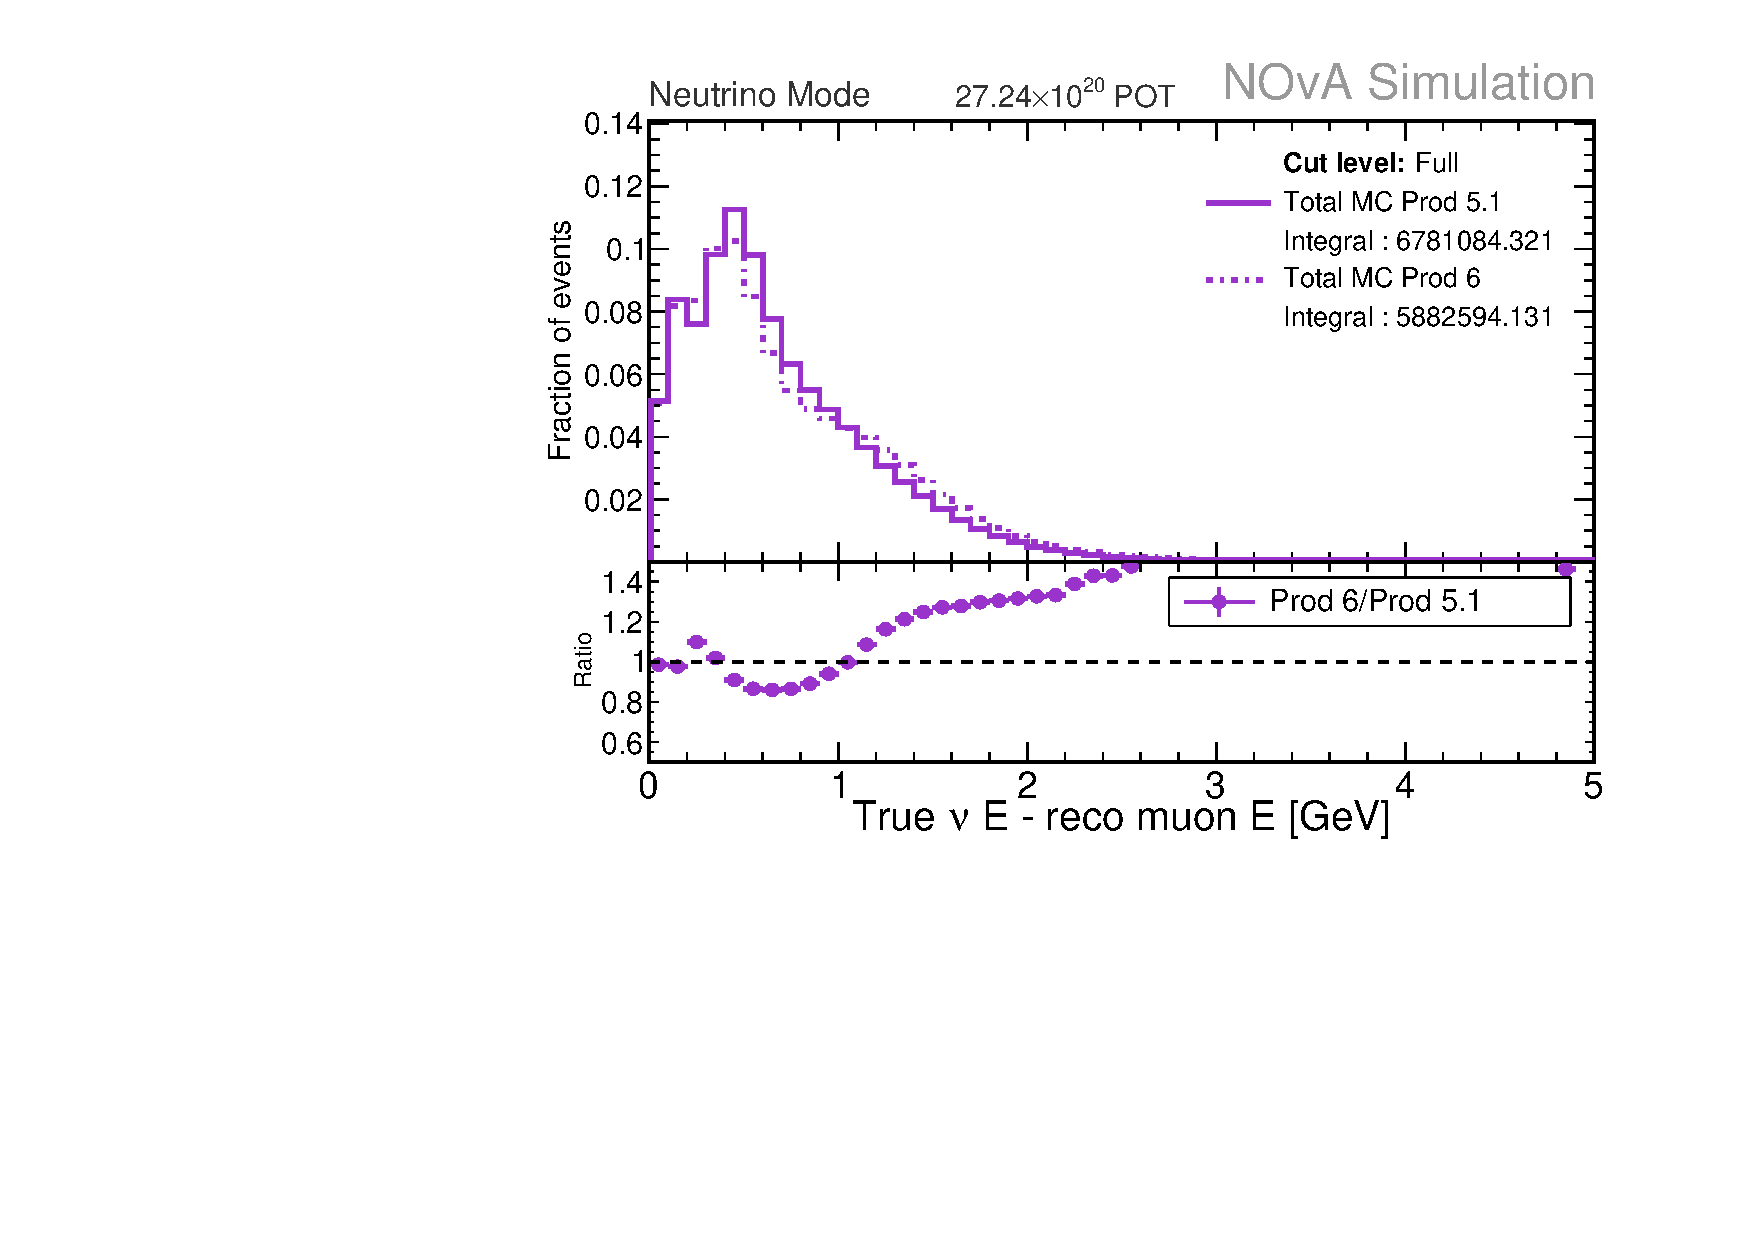
\includegraphics[width=0.7\textwidth]{images-cmurthy/kTrueHadE_Quality_Contain_PID_hadEfracAllQs_pTfracAllQs_numu_fhc_MC.pdf}%
    }{%
        \fbox{\parbox[c][0.25\textheight][c]{0.7\textwidth}{\centering Example image placeholder from \texttt{images-cmurthy/example-image.png}}}%
    }
    \caption{True hadronic energy for Production 6 vs Production 5.1, where the higher average Production 6 hadronic energy can be seen. This validation uses the Production 5.1 energy estimator on both Production 5.1 and Production 6 MC.}
    \label{fig:hadEtrue}
\end{figure}

\section{Production 5.1/6 Data/data comparisons}

All definitions used only include runs and subruns present in both productions. The data/data comparisons show somewhat similar behavior to the MC/MC comparisons, although the ratios are slighly different.\cite{2026-06-08-prod6-validation}

\begin{figure}[htbp]
    \centering
    \IfFileExists{images-cmurthy/example-image.png}{%
        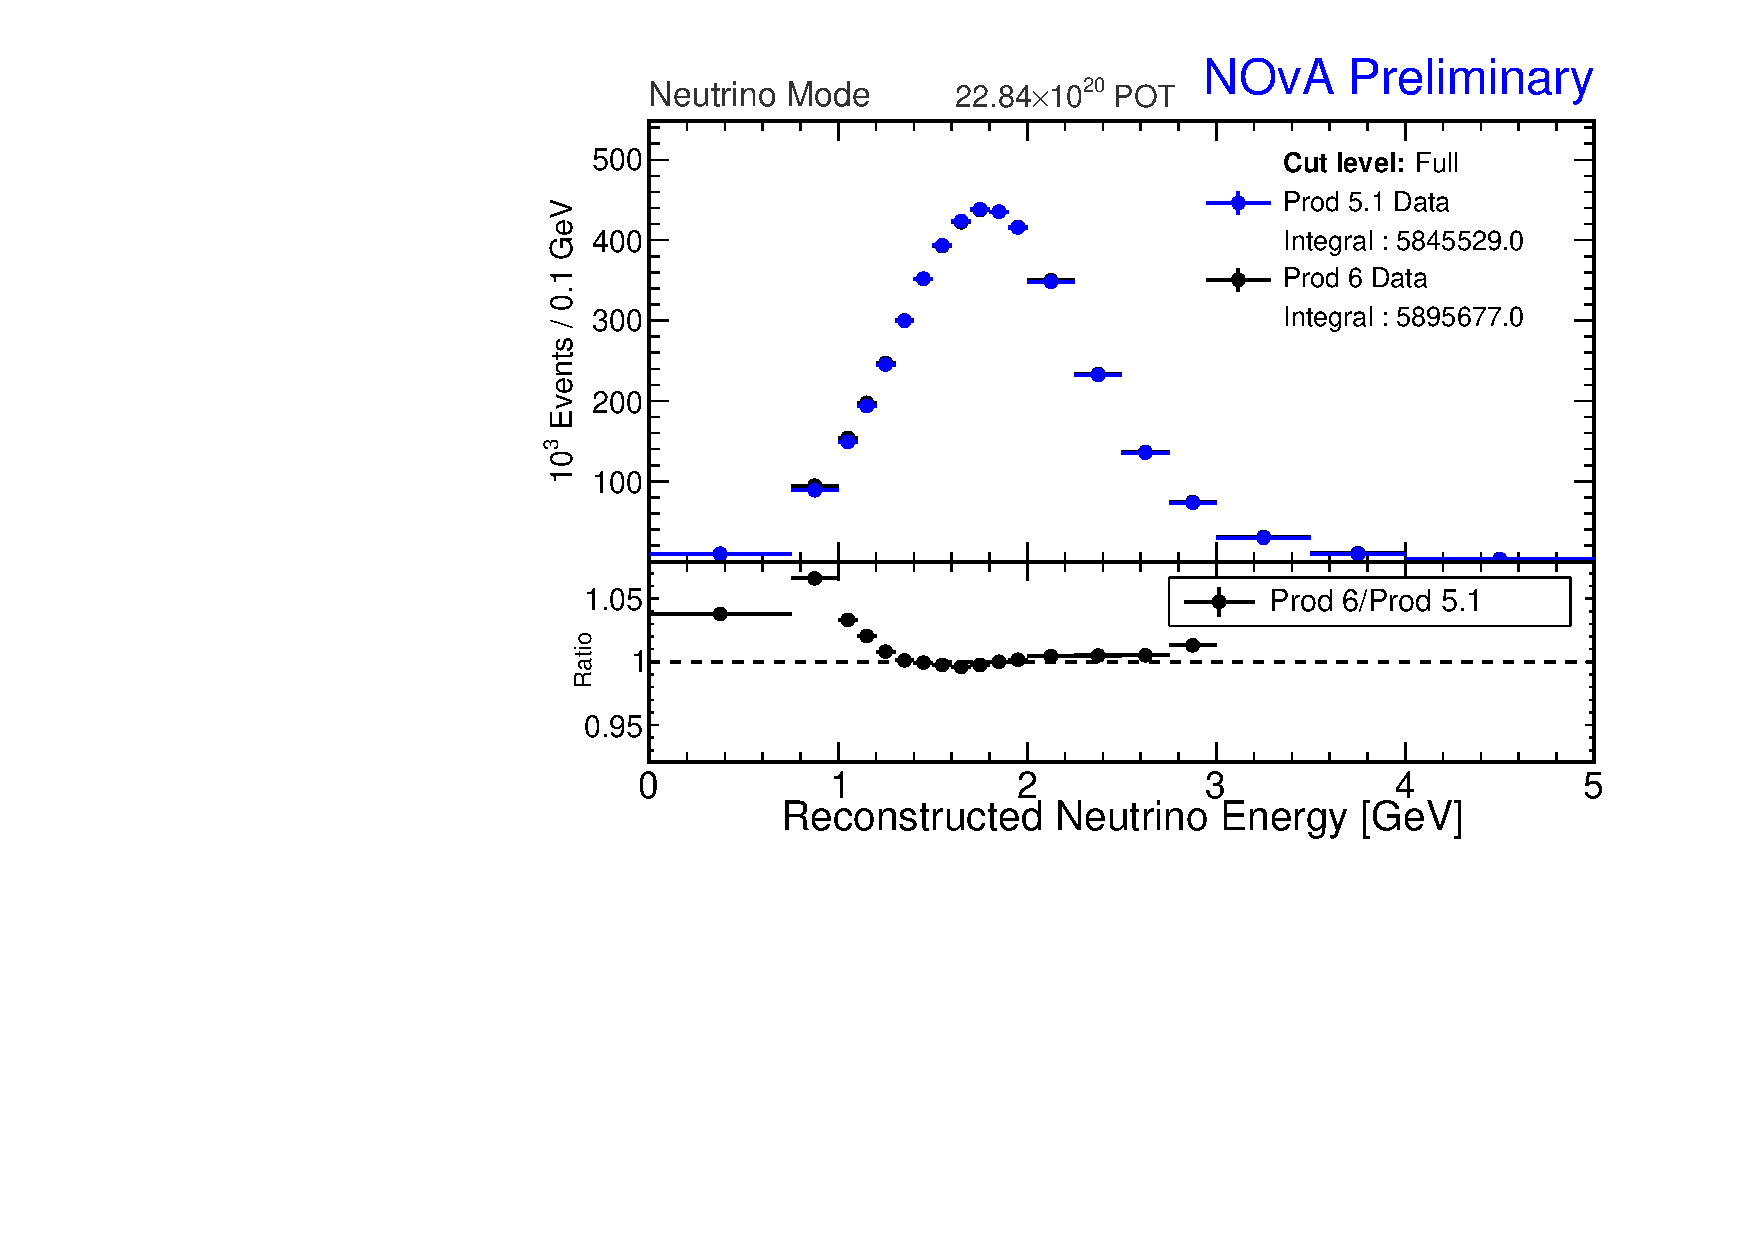
\includegraphics[width=0.7\textwidth]{images-cmurthy/CCE_Quality_Contain_PID_hadEfracAllQs_pTfracAllQs_numu_fhc_Data.pdf}%
    }{%
        \fbox{\parbox[c][0.25\textheight][c]{0.7\textwidth}{\centering Example image placeholder from \texttt{images-cmurthy/example-image.png}}}%
    }
    \caption{Reconstructed neutrino energy for Production 5.1 vs Production 6 data.}
    \label{fig:recoE}
\end{figure}

In data, we also see a slight increase in events in Production 6, particularly at low energies, related to an increase of the number of muons reconstructed with lower energy (see Figure \ref{fig:recoE}). The mean of the muon energy per hit distribution shifts very little (from 16.79 MeV to 16.81 MeV), although the change is more visible at higher hadronic energy fraction quartiles~\cite{2026-06-08-prod6-validation}\cite{2026-07-06-prod6-validation}. We saw also a slight increase in the hadronic energy fraction and a hadEfrac quartile-dependent decrease in the muon $P_T$ fraction, with a larger change in Quartile 4 than Quartile 1~\cite{2026-06-08-prod6-validation}.

\begin{figure}[htbp]
    \centering
    \IfFileExists{images-cmurthy/example-image.png}{%
        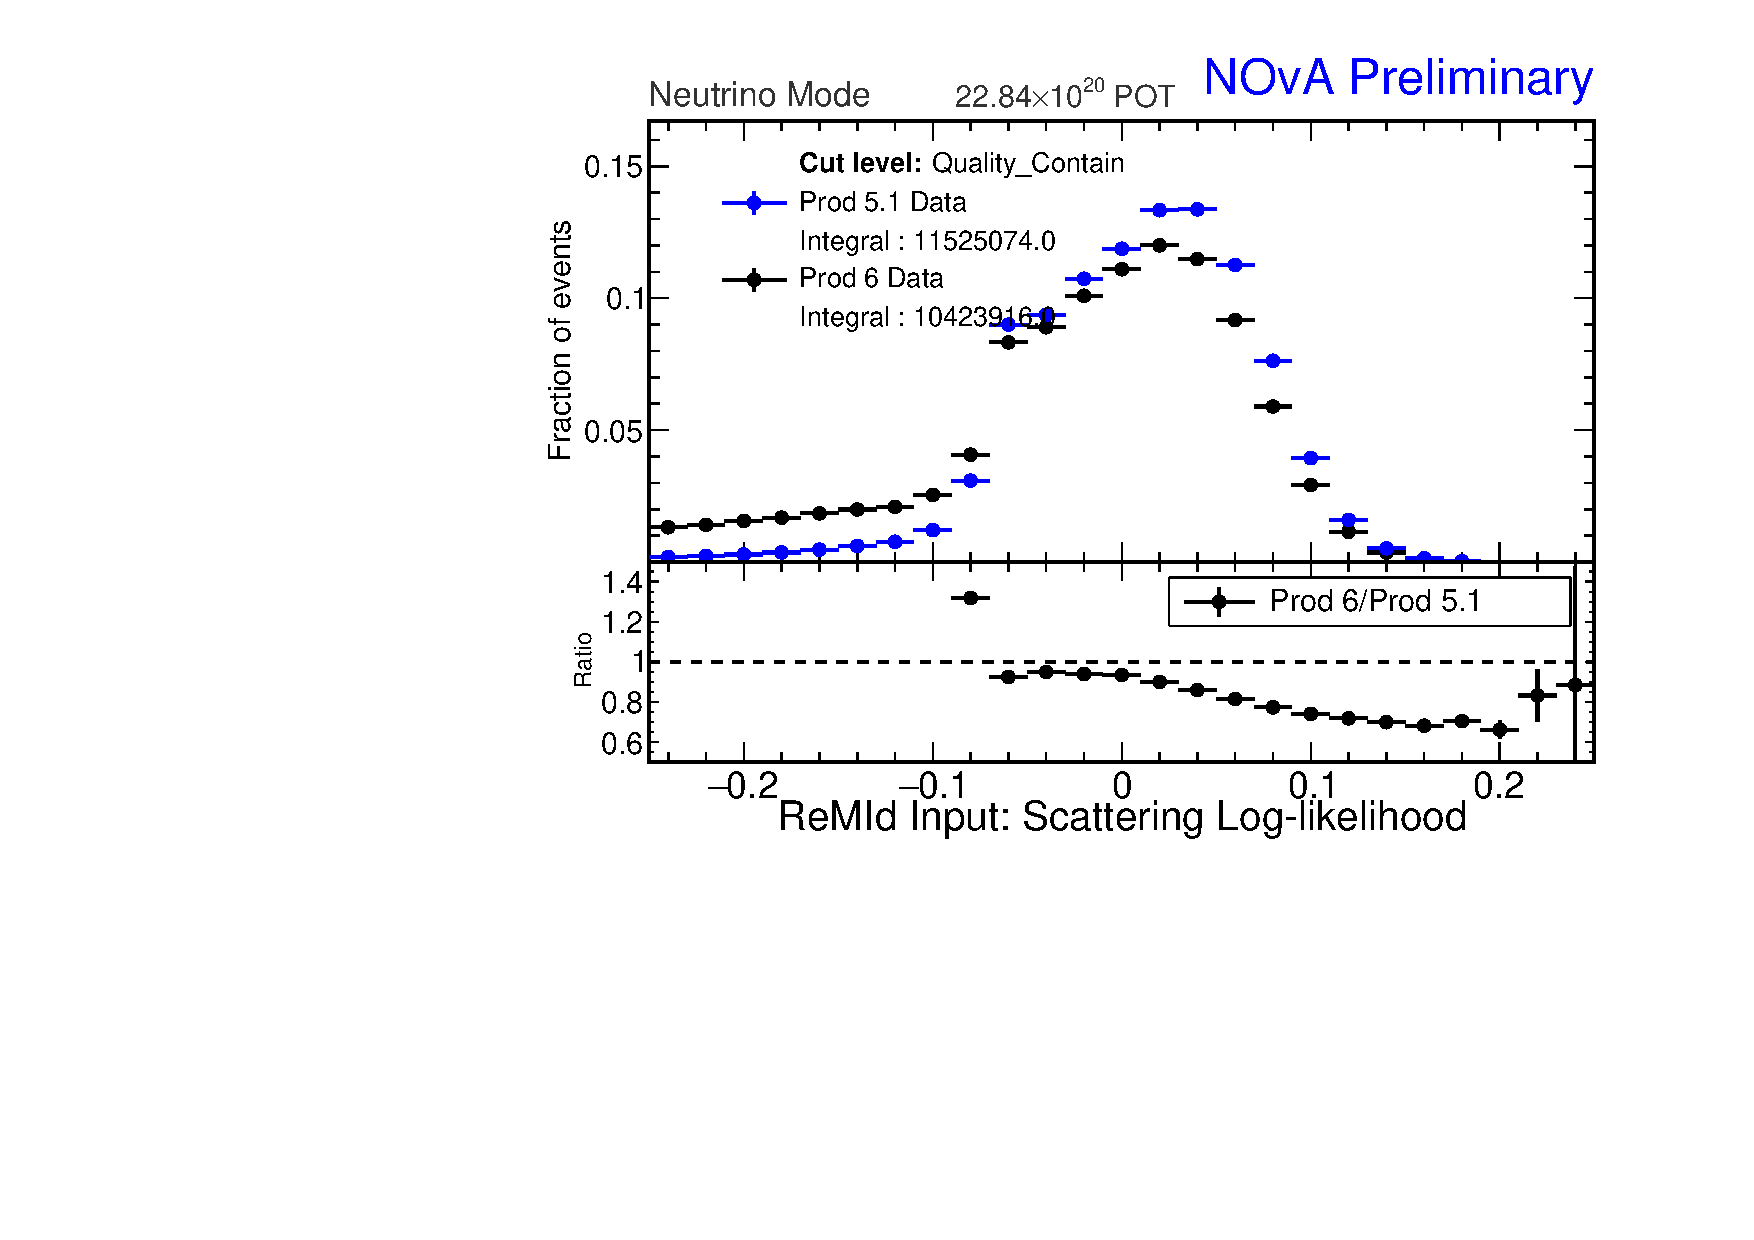
\includegraphics[width=0.7\textwidth]{images-cmurthy/scatLL_Quality_Contain_hadEfracAllQs_pTfracAllQs_numu_fhc_Data.pdf}%
    }{%
        \fbox{\parbox[c][0.25\textheight][c]{0.7\textwidth}{\centering Example image placeholder from \texttt{images-cmurthy/example-image.png}}}%
    }
    \caption{ScatLL variable for Production 5.1 and Production 6 at the Quality Containment cut level for Production 5.1 and Production 6, where the larger tail of Production 6 is clearly visible.}
    \label{fig:scatLLcontain}
\end{figure}

The next major change observed was in the ReMID variable \texttt{ScatLL}, which develops a large tail in Production 6 not found in Production 5.1 (see Figure \ref{fig:scatLLcontain}). The cause of this was found to be a change in the behavior of the $\arccos$ function between ROOT versions where $\arccos$ of any number greater than 1 was returned as $NaN$ instead of 0, causing many tracks to get a very low likelihood score for their scattering angles. As the other ReMID variables showed very little change, the generally lower ReMID values of tracks overall come from this bug~\cite{2026-06-08-prod6-validation}.



\bibliographystyle{unsrtnat}
\bibliography{summary-cmurthy}

\end{document}
